\subsection{Sample Data}
Sample data used for showing the results by Physio Denoise includes 
resting state fMRI data, structural MRI data, PPG data and respiratory data.
Data includes one male subject and is collected in Stockholm University Brain Imaging Centre (SUBIC).

The MRI data is acquired by Siemens 3T with 1.7s of TR. 
Physiological data is acquired with Biopac with 
sample frequency of 10000Hz.

\subsection{Results from Physio Denoise}

From three main steps of Physio Denoise, intermediate variables are saved as outputs for analysis.
To simplify the output lists, the main outputs in each step from Physio Denoise are listed as below.
\\


\begin{forest}
    for tree={
      font=\ttfamily,
      grow'=0,
      child anchor=west,
      parent anchor=south,
      anchor=west,
      calign=first,
      edge path={
        \noexpand\path [draw, \forestoption{edge}]
        (!u.south west) +(7.5pt,0) |- node[fill, inner sep=1.25pt] {} (.child anchor)\forestoption{edge label};
      },
      before typesetting nodes={
        if n=1
          {insert before={[,phantom]}}
          {}
      },
      fit=band,
      before computing xy={l=15pt},
    }
  [Output directory
    [Step1 Preprocess
      [Figures of pipeline and data-flow]
      [<motion correction>
        [corrected NII data]
        [translation and rotations]
        ]
    ]
    [Step2 Regressors
      [MRI pulses csv]
      [regressors csv]
      [respiration histogram]
    ]
    [Step3 Denoise
      [designed matrix]
      [statistical z-maps]
      [denoised NII data]
      [clusters and ROI]
    ]
  ]
\end{forest}

First, the z-maps from results of sample data are meaningful to inspect the ROI of physiological noise.
In Physio Denoise, a threshold of 2 is applied to all z-maps. And in default the order of Fourier
expansion is set to be $2$, which indicates 4 regressors for both cardiac and respiratory signals.

Here, results of sample data will show the ROI regions by Physio Denoise. In Fig. \ref{fig:zmap},
eight z-maps are showing the physiological noise related regions.

\begin{figure}[htp]
  \centering
  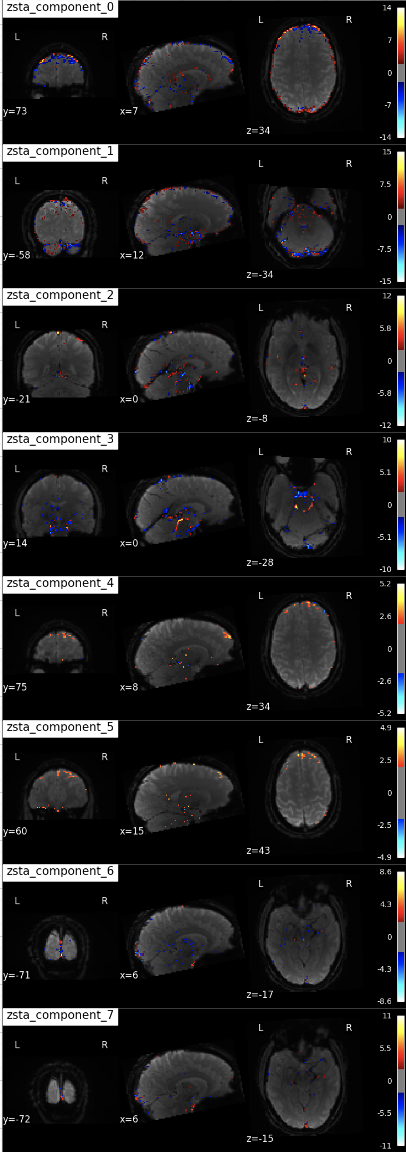
\includegraphics[width=0.8\columnwidth]{Figures/z-map.jpeg}
  \caption{Eight components from Z maps. Components 0-1: 1st order of respiration; Components 2-3: 1st order of cardiac;
  Components 4-5: 2nd order of respiration; Components 6-7: 2nd order of cardiac signal}
  \label{fig:zmap}
\end{figure} 

Component 0 and 1 come from the 1st order of Fourier expansion of respiratory signal.
From z-maps of component 0 and component 1, the highlight mainly locates on the edge of skull. 
It indicates that the signals in the highlight part are highly correlated to respiratory signal. Moreover,
the signal on the edge of brain is less likely to be the neuronal signal. So that it is considered to be
the respiratory noise from fMRI.

Component 2 and 3 come from the 1st order of Fourier expansion of cardiac signal.
From z-maps of component 2 and 3, the highlight part mainly lies in the middle and back of the head.
Especially in the z-map of component 3, the highlight in the middle seems to be connected in a circle line, which is 
interpreted as circles of Willis. On the back of brain, the blood circulation in transverse sinus
could be reflected in z-map. A schematic diagram of veins in brain is shown in Fig. \ref{fig:brain}.

The components from the 2nd order are of less contrast in z-maps, but the regions of highlight
are similar to those of 1st order.

\begin{figure}[htp]
  \centering
  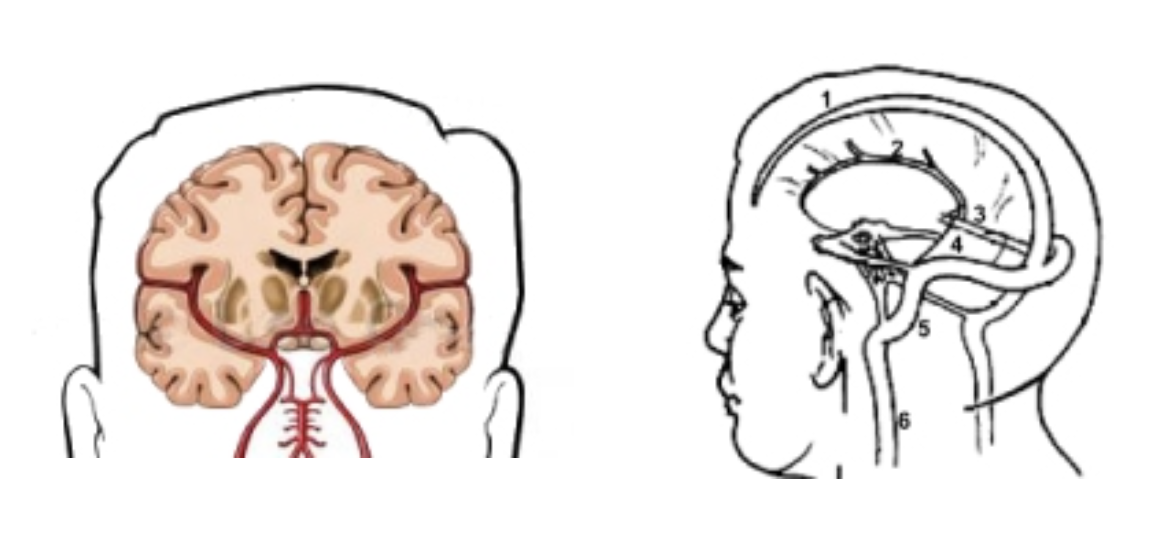
\includegraphics[width=\columnwidth]{Figures/brain.jpeg}
  \caption{Structure of veins inside brain. 1. Superior sagittal sinus; 2. Inferior sagittal sinus;
  3. Straight sinus; 4. Transverse sinus; 5. Sigmoid sinus; 6. Internal jugular vein   }
  \label{fig:brain}
\end{figure} 

Besides the ROI regions of high contrast for each component, clusters are extracted to show the region,
temporal signals and frequency spectrums. In Fig. \ref{fig:clusters}, raw signals, predicted noise signals and 
denoised signals of each cluster are shown in the 1st row.




\begin{figure}[htp]
  \centering
  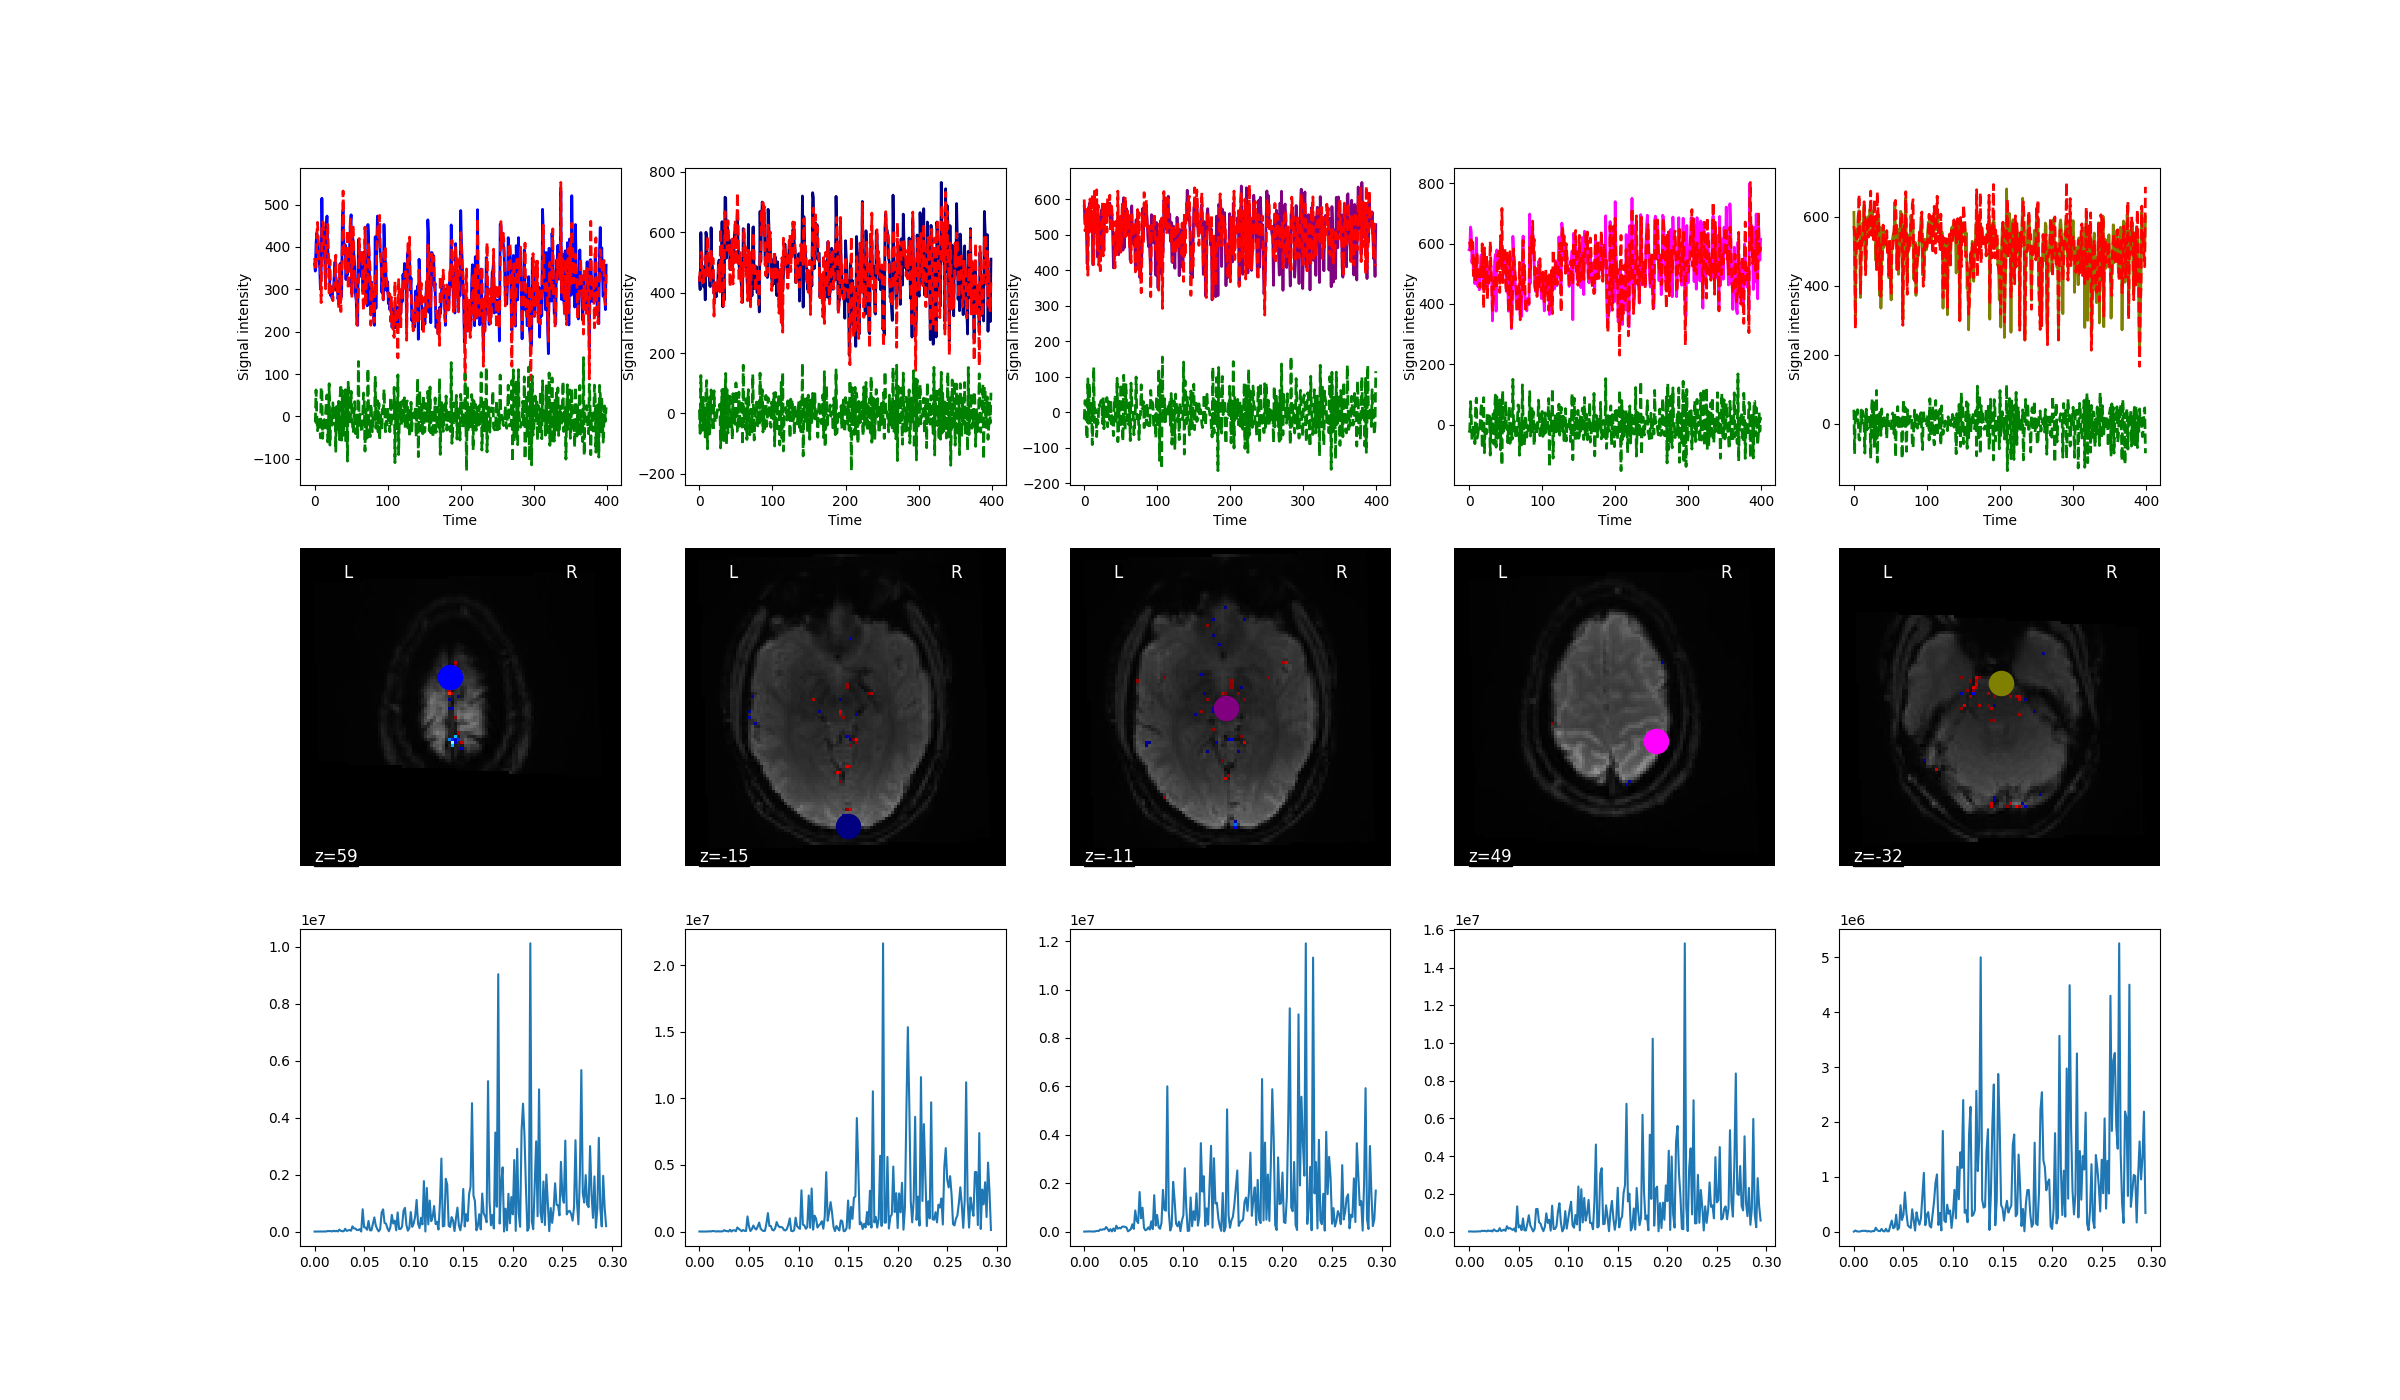
\includegraphics[width=0.9\columnwidth]{Figures/clusters.png}
  \caption{Five Clusters from components. In the 1st row, each graph includes raw BOLD signal(Red), predicted noise signal(Green) and 
  denoised signal. In the 2nd row, it shows positions of each cluster. In the 3rd row, frequency spectrums are of predicted noise signals.}
  \label{fig:clusters}
\end{figure} 





